\documentclass[
  journal=largetwo,
  %manuscript=review,
  year=2025,
  volume=37,
]{cup-journal}

\input{preamble.tex}
\input{math_commands.tex}

\addbibresource{references.bib}

\title{Double descent, and statistical learning/physics}

\author{Bui Gia Khanh}
\affiliation{Department of Physics, Hanoi University of Science, Vietnam National University, Hanoi Vietnam}
\email[Bui Gia Khanh]{fujimiyaamane@outlook.com}

\author{Luong Van Tam}
\affiliation{Department of Physics, Hanoi University of Science, Vietnam National University, Hanoi Vietnam}
% \alsoaffiliation{Joint first authors}

\author{Dang Tri Trung}
\affiliation{Monash University, Department of Computer Science, Melbourne, Australia}

%\author{Daud Shahbaz}
%\affiliation{COMSATS University Islamabad, Islamabad, Pakistan}

%\addbibresource{references.bib}

\keywords{Statistical learning theory, double descent, deep learning, computational complexity theory, complexity theory, statistical physics, spin-glass models, theoretical physics} %% First letter not capped

\begin{document}
\begin{abstract}
    The analysis of learning action, machine learning and related practices in the field theoretically has been made by utilizing Computational Learning Theory (CoLT) \cite{10.1145/1968.1972} and Statistical Learning Theory (SLT) \cite{Vapnik1999-VAPTNO}. These two theories, while overlapped, provides a general framework in analysing and justifying learning actions and learning model constructions, aiding in the formation of modern practices. One of the famous insight using such framework is the \textit{bias-variance tradeoff} \cite{6797087}, which states that model complexity and generality inversely affect each other, thus guarantee the need for a safe bracket between them. However, recent literatures, \cite{belkin_reconciling_2019} has indicated the fallout of such dilemma by the new phenomenon called \textit{double descent}, where there exists an interpolation threshold that renders the current statistical justification for bias-variance inconsequential to a given region. Various `anomaly' has also been detected similarly, with varying degree of sophistication and potential.In this paper, we would like to review through progress made in this particular field of research, and the phenomena potential explanations up until now. 
\end{abstract}

The modern machine learning landscape is dominated and guaranteed by the foundation of theoretical machine learning, specifically computational learning theory (CoLT) and statistical learning theory (SLT). The theory of machine learning and its modern practice has been developed and researched, of a substantial portion by empirical and heuristic approach, either by advancing new practices, architectures or by try-and-test modification. From its early onset of a regression estimator $\theta(x,y)$ on the linear regression problem, machine learning has developed substantially. Certain model concept with great successes includes regression-classification model, Bayesian modelling, generative learning model, support vector machine, Gaussian processes, and more. Of all such, the more formal and complex model architecture created, is the concept of a \textit{neural network}. With increasingly sophisticated architecture, heuristic approach become popular, the fast-paced advancement of the field comes with new method, new results, new observations, and its far-reaching application which led to even bigger and larger scale deployment, there has been questions about the formation and status of a theoretical ground, a rigorous matter on the side of \textbf{theoretical machine learning}.

While rigorous and well-formulated in a sense, classical and theoretical machine learning was dwarfed by the modern advancement of machine learning as a whole, leading to several anecdotal problems regarding the interpretation of phenomena, the re-evaluation of the theory to fit the more updated analysis, and explanation to more sophisticatedly designed system. This and many more, plus as present, many of such advancements and improvements are heuristic, and the general theory and conceptual understanding remain limited, led to the choice to often opt for analogies and empirical workaround. Ultimately, this resulted in multiple `failures' in explaining, interpreting, and predicting behaviours of new phenomena appeared in the modern landscape of machine learning. While there exists novelty of analysis, and different theoretical schemes to analyse such, particular problems remain in the form of irregularity and conflict of interpretations between frameworks. 

We hope to use the theory of statistical physics, as seen of widespread usage in the history of development of artificial intelligence and computational method of such, as seen from \cite{hopfield1982neural,amit1985spin,gardner1988optimal,seung1992statistical,mezard1987spin,mezard2009information,engel2001statistical,advani2013statistical,bahri2020statmech,mehta2014exact,advani2017high,li2021statmechdeep,cavity_tutorial_delFerraro}, with mentions of such statistical mechanics application in \cite{roberts2021principles}. Some of those statistical learning schemes resulted in the works of G. E. Hinton on the variation of neural network called \textbf{Boltzmann machine}, as seen of \cite{ackley1985learning} and \cite{hinton2012practical}. Nevertheless, such question remains if the statistical scheme overreached of its current applicable form, to indict misleading or only limited improvement and interpretability onto a machine learning and in general an artificial intelligence system dynamics. In addition, assumptions and structural constraints, such as those incurred on Boltzmann machines for it to facilitate an environment interpretable of statistical physics remains a question of interest\footnote{It is widely concern of the fact that there exists many interpretations of machine learning mechanics under different formal language, or application-biased one. Such is, for example, information theoretic, as seen of \cite{RussoZou:2016:InformationTheory,XuRaginsky:2017:InfoGen}, categorical theoretic approaches, of \cite{Manin_2024}, and accordingly, control theory, topological learning, graph theoretical, and statistical physics. While interesting as to illuminate the same problem under different lens, it is troubling of the messiness in such approach, as different theories claim different hypothesis, principles, theorems and axioms. Furthermore, it is of questionable intent to simply forgive the account of applying one's field on another --- there exists the fundamental \textit{domain bias} --- of which as can be seen in statistical physics, for certain event to be applicable of using statistical law, one either must adapt the notion and introduce analogous notion (like temperature and relative model diffusing entropy), or restricting the domain, structure, range of expression, and mechanics --- similar to how Boltzmann machines are. Additionally, applying without care gives increasingly large amount of domain bias, as concepts typically seen and assumed of a system in one theory might interject wrongfully, or simply conflict, narrow down the applicable range of such application, or in the worst case, invalidate the result.}. Even with such problems, we would like to retain the view that statistical physics can be indeed used to interpret double descent, though with such phenomena, requires extreme cautions of logical assumptions and modelling setting.  
\section{Foundational works}

On itself, the phenomena \textit{double descent} has been investigated somewhat comprehensively, firstly introduced by \cite{belkin_reconciling_2019}, which gives it distinctive saddle escape illustration. Further analysis was made by several literatures, particularly attributed the existence of double descent to the concept of model complexity and inductive bias, and potential explanations of such. \cite{nakkiran_deep_2019} expanded the phenomena into deep neural network models. Their conclusion is reached by considering the perturbation of a learning procedure $\mathcal{T}$ on the effective model complexity $\mathrm{EMC}_{\mathcal{D},\epsilon}(\mathcal{T})$ defined in the paper, separating the eventual phenomena into regions of observations, thereby in one way or another, predicting the tendency of double descent. This is also the first, arguably, "concise" definition of double descent, even though its nature is an empirical definition, including the notion of model complexity. Recently, there is also the Neural Tangent Kernel (\cite{Jacot:2018:NTK}) which can be used to explain double descent, however further researches are still required. Preliminary works are done by \cite{lafon_understanding_2024}, \cite{schaeffer_double_2023}, and \cite{liu2023understandingroleoptimizationdouble} on the role of optimization in double descent. \cite{davies_unifying_2023} attempted to unifying grokking with double descent, theorized a possibility of similarity during the generalization phase transition of the inference period, and \cite{olmin2024understandingepochwisedoubledescent} attempted to explain epoch-wise double descent within the model of two-layer linear network. However, it is mentioned that it can also be expanded into deep nonlinear networks. 

Further literatures on double descent varies, but fairly new, ever since their discovery articles in \cite{belkin_reconciling_2019} and \cite{nakkiran_deep_2019}. Since then, we have \cite{shi2024homophilymodulatesdoubledescent,schaeffer_double_2023,quetu_can_2023,lafon_understanding_2024,neal2019biasvariancetradeofftextbooksneed,davies_unifying_2023,quetu_can_2023-1,liu2023understandingroleoptimizationdouble,mei2020generalizationerrorrandomfeatures,mei2019generalization,adlam2020understandingdoubledescentrequires,transtrum2025egaddoubledescentexplained,liu2021kernelregressionhighdimensions,allerbo2025changingkerneltrainingleads,pezeshki2021multiscalefeaturelearningdynamics,brellmann2024on,nakkiran2019moredata,mei2019randomfeatures,heckel2020early,nakkiran2020regularization,Belkin_2020,Yang_2024,spiess2023doublesingledescentcausal,nakkiran2021optimalregularizationmitigatedouble,zhang2024manipulatingsparsedoubledescent,cherkassky2024understand,nakkiran2019datahurtlinearregression}. An even more exotic version of double descent, dubbed \textit{triple descent} (or more), is discovered in \cite{d_ascoli_triple_2020}. 

\section{Foundation of learning theory}

Most of the paper will argue about different features of statistical learning theory (\cite{Sterkenburg_2024,Vapnik1999-VAPTNO,STL_Hajek_Maxim_2021}). It is then imperative to discuss the background setting of such. We are given the observations, or dataset of the form $\mathcal{S}=(\mathcal{X},\mathcal{Y})\subset \mathbb{R}^{n}\times \mathbb{R}^{m}$, of all 2-tuple pairs, assumed to be sampled or observed and governed by a distribution $\mathcal{D}$. 

\begin{equation*}
    \mathcal{S} = \{ (x_1,y_1), (x_2, y_2),\dots(x_n,y_n) \} \subset \mathcal{X}\times \mathcal{Y}
\end{equation*}
The dataset is assumed to be i.i.d. sampling according to $\mathcal{D}$, which is unknown by the priori. Hence, we have the first set of assumption. 
\begin{assumption}
The observational space is governed by a particular sampling distribution $\mathcal{D}$, for fixed $y$-response according to the concept $c\in \mathcal{C}$. The sampling process is further assumed to hold no further structure, hence is \textit{identically and independently distributed} (i.i.d.). 
\end{assumption}

The learning problem is then formulated as followed. Given the machine learning model expressed a hypothesis $h$ of the hypothesis class $\mathcal{H}$, the learning theory aims for creating a procedure to learn either elements of the concept class $\mathcal{C}$ of all concepts $c: \mathcal{X}\to \mathcal{X}$, or the function class $\mathcal{F}$ of all functions $f: \mathcal{X}\to \mathcal{Y}$, which is usually set to $\{0,1\}$ or $[0,1]$. This distinction is trivial, hence, if it is clear, we will talk about the concept class $\mathcal{C}$ only as representative form. The learner $\mathcal{L}(h)$ consider the set of possible hypothesis $\mathcal{H}$, in which might not coincide with $\mathcal{C}$. It receives a partial image of sample $S=(x_{1},\dots,x_{2},\dots,x_n)$ drawn i.i.d. according to $\mathcal{D}$ as well as the label $(c(x_1),\dots,c(x_n))$. This constitutes the dataset $\mathcal{S}$, which are based on specific concept $c\in \mathcal{C}$ for the hypothesis to learn. The task is then to use (or \textit{extract}) meaningful information to select a hypothesis $h_{S}\in \mathcal{H}$ that accurately mimic $c$, with marginal error $\Theta$. The notation $h_{S}$ stands for all hypothesis that can be inferred from the range of the dataset (the first argument, $\mathcal{X}$). 

The marginal error $\Theta$ is considered of two parameters, the empirical error $\hat{R}(h)$ and the generalization error $R(h)$. We give the following definition of them. 

\begin{definition}[Empirical risk]
    Given a hypothesis $h\in \mathcal{H}$, a target concept $c\in \mathcal{C}$, and a sample $S=(x_{1},\dots,x_{m})$. For some particular $\epsilon>0$, the \textbf{empirical error} or \textit{empirical risk} of $h$ is defined by\begin{equation}
        \hat{R}_{S}(h) = \underset{x\in S\sim\mathcal{D}}{\mathbb{P}} [\ell\{h(x),c(x)\}\geq \epsilon] =\frac{1}{m} \sum_{i=1}^{m} \ell\{h(x_i),c(x_i)\}
    \end{equation}
\end{definition}

The generalization risk is then defined as the extension of the empirical risk, of which instead of being evaluated on the set $\mathcal{S}$, it is evaluated on arbitrary infinite density sample space. The notation for the risk calculation can also be $R_{\mathcal{S}}$ instead, of which the need is to classify the set of which it is evaluated from. 

\begin{definition}[Generalization risk]
    Given a hypothesis $h\in\mathcal{H}$, a target concept $c\in\mathcal{C}$, and an underlying distribution $\mathcal{D}$ on $\mathcal{X}$. For some particular $\epsilon>0$, the generalization error or \textit{risk} of $h$ is defined by
    \begin{equation}
        \begin{split}
          R(h) 
          &= \underset{x\sim\mathcal{D}}{\mathbb{P}} [\ell\{h(x),c(x)\}\geq \epsilon]\\
          &= \underset{x\sim\mathcal{D}}{\mathbb{E}}[\ell\{h(x),c(x)\}]\\ 
          &= \int_{x\in \mathcal{D}} \ell\{h(x),c(x)\} \: dP(x)
        \end{split}
    \end{equation}
\end{definition}

In essence, the empirical risk measure the hypothesis to observation error, and the generalization risk captures the difference of the hypothesis to the actual concept. Notice that by doing this, we have implicitly assumed that the observations and the concept is not the same thing, under the majority of scenarios. For the observations to be \textit{approximately equal} or sufficiently captures the concept, there then would have to be various criteria to fulfil. 
For fixed $\mathcal{H}$, for fixed and sufficiently large $\mathcal{S}$, and no observation (data) errors, the empirical risk is the generalization risk. These two measures between $h$ and $c$ constitute the learning problem, which can also be separated into both cases - either empirical learning or generalization learning, one to minimize $\hat{R}(h)$, and one to minimize $R(h)$. Here, we emphasize such hierarchy by defining the generalization goal as the \textbf{nested criteria} for empirical risks minimization. 

\begin{definition}[Empirical learning problem]
    We present the formal form of the empirical learning. Suppose we have a \textbf{target}, $c\in\mathcal{C}$, where $\mathcal{C}$ is an arbitrary concept class that captures targets of the same type. Suppose we are provided a set of observations $\mathcal{S}$. The problem is to use certain algorithm $\mathcal{A}$ using $\mathcal{S}$, to obtain a hypothesis $h^{*}$ for a fixed $\mathcal{H}$ such that: 
    \begin{equation}\label{eq:lp1}
        R(h^{*}) = \min_{h\in\mathcal{H}} \hat{R}(h) = \min_{h\in\mathcal{H}} \underset{x\sim\mathcal{D}, x\in \mathcal{S}}{\mathbb{E}}\:\ell\{h(x),c(x)\}
    \end{equation} 
\end{definition}

The generalization best $\bm{h}$ is also called in literature as the \textit{Bayes model}, such that it reduces the Bayes risk that is the infimum of the generalization risk, $R^{*}=\inf_{h\in \mathcal{H}}R(h)$. The hypothesis $h^{*}$ is often called the \textit{empirical best}, for it being the minimal, finite hypothesis of the lowest loss evaluation on the entire observation space $\mathcal{S}$. There exists no certified assumption regarding whether $h^{*}$ aligns with the minimal generalization error.

\begin{definition}[Generalization learning problem]
    We present the formal form of the generalization learning problem. Suppose we have a \textbf{target}, $c\in\mathcal{C}$, where $\mathcal{C}$ is an arbitrary concept class that captures targets of the same type. Suppose we are provided a set of observations $\mathcal{S}$. Supposed we have an algorithm $\mathcal{A}$ that for fixed hypothesis space $\mathcal{H}$, \eqref{eq:lp1} holds true. The problem is to use certain algorithm $\mathcal{A}'$ such that, under limited availability, to obtain $\bm{h}$, satisfies: \begin{equation}
        R(\bm{h}) = \min_{h\in \mathcal{H}} R(\bm{h}) \leq \{\epsilon\}, \quad \epsilon > 0 
    \end{equation}
    For a set of risk bounds $\epsilon$. If the setting is deterministic, then there exists $\epsilon=0$ accordingly. 
\end{definition}

Then, we can partially say that generalization problem is an advancement from empirical solution. As such, empirical solution imposes the observed concept, and not the concept itself. This is reflected in modern machine learning landscape, by modelling the concept as distributions, and then using notions such as KL-divergence to measure such relative disparity. 

The process of generalization goal can be, described in certain form as the global optimization objective in which empiricism can obtain from reasonable set of assumptions and conditions. The following algorithmic framing indeed aims to focus and extradite such sense of operational goal. 

\RestyleAlgo{ruled}
\SetKwComment{Comment}{}{}
\SetKwBlock{Objective}{Objective}{}
\begin{algorithm}[htb]
    \renewcommand{\algorithmcfname}{Optimization problem}
    \caption{Empirical-generalization learning dynamics (non-proxy)}
    \KwData{$(x_{i},y_{i})\in\mathcal{S}, \Gamma \supset \mathcal{S}$, objective $\ell(y,f(x))$, $\nabla(\cdot)$ differentiable gradient field on $\ell$.}
    \KwResult{Expected optimized model to the minimal error on the objective $\ell(\cdot,\cdot)$, dependent on $\mathcal{S}$.}
    \Begin
    {
        $\Gamma\supset \mathcal{S}$, the general set\;
        $R(\cdot),\hat{R}(\cdot)\gets\ell$ as objective functional\;
        \For{Fixed $\mathcal{H}$, with $h\in\mathcal{H}$, for $\epsilon > 0$}{
            Find $h\to \bm{h}'$, using algorithm $\mathcal{A}$ for minimization objective, such that 
            \begin{equation}
                \mathcal{A}\left(\min_{h\in\mathcal{H}} \hat{R}_{\mathcal{S}}(h) + R(h)\right) \leq \epsilon 
            \end{equation}for procedure $\mathcal{A}(\cdot,\cdot)$ of structural constraints.\;
        }
    }
    \Return{Optimized model $h$ on arbitrary objective space $(\ell,\nabla)$.}
    \label{algo:algo_optim_ideal}
\end{algorithm}

These two stages of learning procedure comes of as the intrinsic design of machine learning setting. As opposed to interpolation, where empirical learning problem would have to be put into first priority to achieve the best possible point-through model, machine learning leans on approximation more and a separated criterion that is only visible in the learning setting - the fact that we are using $c'$ to extract $c$. This disparity is exactly the \textbf{generalization problem}, of which is then also the goal of machine learning, to approximate the general solution using the observed solution. One then can ask what is the difference between the two notions, and when we can guarantee that both will `converge' to the same point. The process of \textbf{model selection} is then the procedure that will optimize $h\in \mathcal{H}$ to a given target fixture, such as the empirical best. 

One of the major assumption or observation from the point of the hypothesis class, is that the hypothesis cannot know the generalization error. Thereby, the more efficient and often used procedure/algorithm in training, is then the \textit{empirical risk minimization} (ERM) method, minimizing only the empirical risk to the empirical best; then, certain measures to `generalize' this heuristically is apprehended on the hypothesis. The process of model selection is also the place that we get the concept of \textbf{bias-variance tradeoff}, and its longstanding form to be a foundational metric on model selection. 

\subsection{Empirical and structural algorithms}

Suppose that for a concept class $\mathcal{H}$, we can then partition it to $\mathcal{H}=\bigcup_{k\in \mathbb{N}} \mathcal{H}_{k}$ for finite $k$ hypotheses. Assume that they satisfy the uniform convergence (\cite{JMLR:v11:shalev-shwartz10a}), which means in the arbitrary path landscape, one can guarantee $\ell$-reduction, of $m$ samples on $\mathcal{S}$ to:

\begin{equation}
    \lim_{m\to \infty} \sup_{\mathcal{D}} \underset{S\sim\mathcal{D}^{m}}{\mathbb{E}} \left[ \sup_{h\in\mathcal{H}} [R(h) - R_{S}(h)] \right] = 0
\end{equation}

Then such is said to be possible as a ruling dynamic when for a learning problem, the empirical risks of hypotheses in the hypothesis class converges to their population risk uniformly, with a distribution-independent rate. The result of this is that a problem then can be considered learnable with the ERM rule, for any given characterization. We state the following definition.\footnote{The reason why $r(\cdot)$ is not characterized in this preliminary section, is because of their uncertainty of effect. Hypothetically, $r(\cdot)$ is an additional structure (bias) of which apply a new gradient field in conjunction to the loss gradient field itself. This addition is uncertain of its content and analysis, since it depends on various stochastic dynamics of the model. We reserve from using regularization for now because of such reason.}

\begin{definition}
    A learning problem is learnable if there exist a learning rule $\mathcal{A}$ and a monotonically decreasing sequence $\epsilon_{cons}(m)$ such that $\epsilon_{cons}(m)\overset{m\to\infty}{\longrightarrow} 0$ and \begin{equation}
        \forall \mathcal{D} , \quad \underset{S\sim\mathcal{D}^{m}}{\mathbb{E}} \left[F(\mathcal{A}(S))-F^{*}\right] \leq \epsilon_{cons}(m),
    \end{equation}
    with $F^{*} = \inf_{h\in\mathcal{H}} R(h)$. A learning rule $\mathcal{A}$ for which this hold is denoted as a universally consistent learning rule. 
\end{definition}

There are certainly a fundamental class of rule or algorithm $\mathcal{A}$ to resolve this particular uniform convergence of classes. One of the major assumption or observation from the point of the hypothesis class, is that the hypothesis cannot know the generalization error. Thereby, one strategy is the \textit{empirical risk minimization} (ERM) method, minimizing only the empirical risk to the empirical best; then, certain measures to `generalize' this heuristically is apprehended on the hypothesis. 

\begin{definition}
    A rule $\mathcal{A}$ is an ERM (Empirical Risk Minimizer), denoted $\mathcal{A}_{ERM}$ if it minimizes the empirical risk $\hat{R}(h)=(1/m)\sum_{c\in\mathcal{C}}\ell(h,c)$, over the observational space $S$, 
    \begin{equation}
        \hat{R}_{S}(\mathcal{A}_{ERM}(S)) = \hat{R}_{S} (h_{S}) = \inf_{h\in\mathcal{H}} \hat{R}_{S}(h) 
    \end{equation}
    Hence, the ERM tries to obtain $\mathrm{ERM}(h') = \argmin_{h\in \mathcal{H}} \hat{R}(h)$. 
\end{definition}

The problem of overfitting still somewhat resides in the setting of the method. Hence, usually, we have an implicit term in addition, called the \textit{regularizer}, of which is as followed. 

\begin{definition}
    A rule $\mathcal{A}$ is an SRM (Structural Risk Minimizer), denoted $\mathcal{A}_{ERM}$ if it minimizes the empirical risk $\hat{R}(h)=(1/m)\sum_{c\in\mathcal{C}}\ell(h,c)$, over the observational space $S$, 
    \begin{equation}
        \hat{R}_{S}(\mathcal{A}_{SRM}(S)) = \hat{R}_{S} (h_{S}) + \lambda r(h)= \inf_{h\in\mathcal{H}} \hat{R}_{S}(h) + \lambda r(h)
    \end{equation}
    of the regularizing term $r(\cdot)$. Hence, the SRM tries to obtain $\mathrm{ERM}(h') = \argmin_{h\in \mathcal{H}} \hat{R}(h)$, while taking into consideration a forcing term $r$, usually defined on the model complexity. 
\end{definition}

Hence, the SRM is inherently stronger than ERM. The regularizer $\lambda r(h)$, in specific case of convex loss landscape and reasonably well-behaved irregularities between domains, and of the structural regularization term $r_{s}(h)=\sum_{i,j}w_{ij}^{2}$ for weights of $ij$ index, then we have that 
\begin{equation}
    \mathrm{ERM}\left(\inf_{h\in\mathcal{H}} \hat{R}_{S}(h), \ell\right) \approx o\left(\mathrm{SRM}\left(\inf_{h\in\mathcal{H}} \hat{R}_{S}(h) + \lambda r(h), \ell + \lambda r(h)\right)\right)
\end{equation}
Where the little-$o$ notation is used for saying of the optimization strength per arbitrary time-similar notion of algorithmic evolution. The reason for this change is because of the restriction domain that $\mathrm{SRM}$ indicted on the model optimization landscape. Effectively, we introduce the structural bias $\lambda r(h)$ that forces the morph of the total loss landscape. In well-behaved case, this is usually effective to a point, however in realistic system and pathological cases, such can lead to the $c'$ approximation in $c$-space, just as we introduced in the reformulation of learning system. In this paper, we would like to presume the ERM method in question as the famous \textit{gradient descent}. We refer to \cite{achlioptas_stochastic_nodate,ruder_overview_2017} for general view of the algorithm, and \cite{zhang_gradient_2019} for a source on particularly gradient descent algorithm on deep learning models. 

\subsection{Overfitting and underfitting}

Following the above framework of statistical probabilistic learning theory, one understanding about the concept of underfitting and overfitting (similar to \cite{James2021}) can be reached, using the notion of \textit{partitioning} of observation space. Such work is typically done because of \textbf{practical condition}, in which the following constraints is applied.
\begin{assumption}\label{assume:cpi_transparency}
    No knowledge of $c\in\mathcal{C}$ is provided. \footnote{Few points need to be said about this assumption. This assumption represents the \textit{worst-case possible} of a system dynamic. From the perspective of a designer, inherent leakage of information can be provided in the design of a model. In such, case we are operating in the mode of a \textit{resource-constrained, closed} game, in which the model with further assumptions of fixed class, operates on. The problem space itself is inherently large and penalize any additional structural changes. If one is to occur, we usually mention it as \textit{implicit bias}, but another name that would be more fitting would be \textit{structural attractor}, after the notion of gradient attractor in chaotic systems.}
\end{assumption}

Without such knowledge, $R(h)$ cannot be computed, accordingly. We specify such approach as \textit{heuristic}, as it is only an approximation, and for better definition, we define it as followed. 

\begin{definition}[Heuristic empirical risk]
  Given a dataset $\mathcal{S}$ of size $m$, supposedly of the concept $c\in \mathcal{C}$, and the hypothesis $h\in \mathcal{H}$, then the \textbf{heuristic empirical risk} take a partitioning $k<m$ with $k/m\geq 1/2$, hence defining the heuristic empirical loss on $k$, denoted $\hat{R}_{k}(h)$. 
\end{definition}

\begin{definition}[Heuristical generalization risk]
  Given a dataset $\mathcal{S}$ of size $m$, supposedly of the concept $c\in \mathcal{C}$, and the hypothesis $h\in \mathcal{H}$. Fixed $\hat{R}_{k}(h)$, for the final optimization of algorithm $\mathcal{A}$, then the \textbf{heuristic generalization risk} take the remaining 2-partition of portion $p=k-m$, hence defining the heuristic generalization loss on $p$, denoted $\hat{R}_{p}(h_{\mathcal{A}})$. 
\end{definition}
The two heuristic definition however, can be noted to not be equal to the true generalization risk - empirical risk pair in reality. Nevertheless, one can then define overfitting and underfitting in such manner. 
\begin{definition}[Underfitting]
  A model $h$ is called \textbf{underfitting} if for a constant $\epsilon > 0$ chosen for the setting, then $\hat{R}_{k}(h_{\mathcal{A}})>\epsilon$, $\hat{R}_{p}(h_{\alpha})> \epsilon$ over the entire observation space. 
\end{definition}
Usually, underfitting is defined to be such that test error is smaller than training error partition, however, we do not think that is a good definition. Especially since, at least in this setting, the empirical error under algorithm $\mathcal{A}$ is reduced to the representative smallest error that $\mathcal{A}$ can achieve on that particular model, within particular setting of $h$, then come the heuristic generalization error. Considering also that $k/m\geq 1/2$, that is, at least the training partition is half of the observation set, then only under very specific case will $\hat{R}_{p}(h_{\alpha})$ be smaller than $\hat{R}_{k}(h)$, statistically speaking. Thence this line of thought also reinforces the idea that both of them will be larger than the threshold $\epsilon$. Usually, heuristically, this threshold of error is $0.3$, normalized. Next, we define the notion of overfitting. 

\begin{definition}[Overfitting]
  A model $h$ is called \textbf{overfitting} if there exists a specific constant $\epsilon>0$ chosen for the setting, such that $\hat{R}_{k}(h)<\epsilon$, $\hat{R}_{p}(h_{\alpha})> \epsilon$ over the entire observation space.
\end{definition}
Namely, this mean that the static learning makes the generalization error worse. This draws the analogy of the student - studying explicitly for the past paper tests, yet unaware of the larger margin of questions in the large set of the test paper pool, leading to subpar performance. Similarly, overfitting is theorized to be fitting too fit to the reduced observation space - hence when it comes to the generalization observation space, it fails within such heuristic. The notion works on the mask of the risks, $\hat{R}_{k}$ and $\hat{R}_{p}(h_{\alpha})$. 

In practice, Assumption~\ref{assume:cpi_transparency} means we cannot have $c\in\mathcal{C}$, or its probabilistic interpretation $\mathcal{D}$ such that $x\sim\mathcal{D}$, or in the extreme non-structured case, $(x,y)\sim \mathcal{D}$. In such case, the typical practical fix relies on the partitioning of the available partitioning space, that is, the empirical-generalization proxy. For large enough singleton count of $|\{(X_{k},Y_{k})\}|$, we assume that $\hat{R}_{\mathsf{Gen}}(h)\approx R(h)$. Thus, the algorithm can be stated in a form as Algorithm~\ref{algo:algo_optim_no_c}.

\RestyleAlgo{ruled}
\SetKwComment{Comment}{}{}
\SetKwBlock{Objective}{Objective}{}
\begin{algorithm}[htb]
    \renewcommand{\algorithmcfname}{Optimization problem}
    \caption{Empirical-generalization learning dynamics (proxy)}
    \KwData{$(x_{i},y_{i})\in\mathcal{S}, y_{i}=\{\pm 1\}$, hinge objective $\ell(y,f(x))$, $\nabla(\cdot)$ differentiable gradient field on $\ell$.}
    \KwResult{Expected optimized model to the minimal error on the objective $\ell(\cdot,\cdot)$, dependent on $\mathcal{S}$.}
    \Begin
    {
        $((X_{1},Y_{1}),\dots)_{n}\gets\mathsf{Partition}_{n}(\mathcal{S})$\;
        $\{(X_{j},Y_{j})\}\gets \mathsf{Train}$\;
        $\{(X_{k},Y_{k})\}\gets \mathsf{Gen}$ for $k\ne j$\;
        \For{Fixed $\mathcal{H}$, with $h\in\mathcal{H}$, for $\epsilon > 0$}{
            (Optimistically) achieve $h\to \bm{h}'$, using algorithm $\mathcal{A}$ for minimization objective, such that 
            \begin{equation}
                \mathcal{A}\left(\min_{h\in\mathcal{H}} \hat{R}_{\mathsf{Train}}(h) + \hat{R}_{\mathsf{Gen}}(h)\right) \leq \epsilon 
            \end{equation}for procedure $\mathcal{A}(\cdot,\cdot)$ of structural constraints.\;
        }
    }
    \Return{Optimized model $h_{\mathcal{A}}$ on arbitrary objective space $(\ell,\nabla)$.}
    \label{algo:algo_optim_no_c}
\end{algorithm}
The assumption above of the generalization set to the generalization truth error is apparent in the usual system theorem, Theorem~\ref{thm:minimalNeu}.
\begin{theorem}[\cite{10.5555/2371238}]\label{thm:minimalNeu}
    For fixed $\mathcal{H}$, for fixed and sufficiently large $\mathcal{S}$, and no observation errors, the empirical risk is the generalization risk: \begin{equation}
        \underset{\mathcal{S}\sim \mathcal{D}^{m}}{\mathbb{E}}[\hat{R}_{\mathcal{S}}(h)]  = R(h)
    \end{equation} 
\end{theorem}

\begin{proof}
    By linearity of the expectation, and the fact that we assume the sample is given i.i.d., we can write: 
\begin{equation}
    \begin{split}
        \underset{S \sim \mathcal{D}^m}{\mathbb{E}}[\hat{R}_S(h)] 
        &= \frac{1}{m} \sum_{i=1}^m 
            \underset{S \sim \mathcal{D}^m}{\mathbb{E}} 
                    \left[ \mathbbm{1}_{h(x_i) \ne c(x_i)} \right] \\
        &= \frac{1}{m} \sum_{i=1}^m 
            \underset{S \sim \mathcal{D}^m}{\mathbb{E}} 
                \left[ \mathbbm{1}_{h(x) \ne c(x)} \right], \\
    \end{split}
\end{equation}
for any \( x \) in sample \( S \). Thus, we result in

\begin{equation}
    \begin{split}
        \underset{S \sim \mathcal{D}^m}{\mathbb{E}}[\hat{R}_S(h)] 
            &= \underset{S \sim \mathcal{D}^m}{\mathbb{E}} 
            \left[ \mathbbm{1}_{h(x) \ne c(x)} \right] \\
            &= \underset{x \sim \mathcal{D}}{\mathbb{E}} 
            \left[ \mathbbm{1}_{h(x) \ne c(x)} \right] \\
            &= R(h).
    \end{split}
\end{equation}
which yields the desired result. 
\end{proof}

This theorem can be transferred to a more generalized conjecture, of which fit the generalized notion of the empirical proxy and so on. 
\begin{conjecture}
    Supposed $\mathcal{H},\mathcal{C}$ are fixed, for $\mathcal{S}$ is the empirical $c^{*}$ for $c\in \mathcal{C}$ the true concept. Then, for algorithm $\mathcal{A}(\cdot,\cdot)$ enforcing minimization apparatus, and the specific objective on the second argument, we have:
    \begin{equation}
        \begin{split}
            &\underset{j\to\infty,\mathcal{S}_{i}\neq\mathcal{S}_{k}}{\mathcal{A}}\left(\min_{h\in\mathcal{H}} \hat{R}_{\mathsf{Train}}(h) + \hat{R}_{\mathsf{Gen}}(h), [\ell]\right)\\
            & \quad \quad \approx \mathcal{A}\left(\min_{h\in\mathcal{H}} \hat{R}_{\mathcal{S}}(h) + R(h), [\ell]\right) + \epsilon_{\mathcal{S}}
        \end{split}
    \end{equation}
    For $\mathcal{S}_{i}\neq\mathcal{S}_{j}$ such that there are only distinct samples, $j$ the observation set size, $[\ell]$ the set of structural or empirical objectives enforced on the problem landscape, and $\epsilon_{\mathcal{S}}$ is the empirical minimum that the algorithm result can achieve assuming sufficient `perfect interpolation'. 
\end{conjecture}

By the end of this section, we would also want to note that we deliberately choose an expression basis of $\mathcal{A}$ via the couple tuplet $(\min, [\ell])$ as a choice for \textit{algorithm-agnostic class} of algorithm satisfies the dynamic only, not just implementations. The algorithm, in certain sense, depends much more on structural assumptions, of which is not accessible via observations but via design, and intrinsic information specified in the observation class itself. This is a requirement for fine-tuning analysis in the long-run, as there exists a myriad of different approaches. 


\section{Bias-variance tradeoff}

In classical sources, \cite{James2021,goodfellow2016deep,STL_Hajek_Maxim_2021,10.5555/2371238,10.5555/2621980}, the principle of bias-variance tradeoff is a classical principle used in the categorization of technique called \textit{model selection}. Specifically, this refers to the progress of choosing the best predictor $h^{*}$ that minimize the generalization error that is the main goal of a particular machine learning model, during the process of training and inference. Originally, the theory that bias and variance often come in to conjunction is \textbf{Estimation theory}, of which there exists an estimator $\hat{\theta}$ that use a set of observations, to estimate the concept, or the underlying mechanics of certain system that outputted the observation set, by the \textbf{probabilistic perspective} - that is, it is governed by appearance by an independently and identically distributed process of parameterized probability $\theta\in \Theta$. Here, parameterized means being expressed by a set, often finite, of parameters, by \cite{LehmannCasella_theory_1998,liam_statistics_2005}. It is only when \cite{6797087} introduced it to machine learning that we have an equivalent structure that is similar to bias-variance in machine learning. 

\subsection{Precursor (\cite{6797087})}

The original definition of bias-variance tradeoff by \cite{6797087} is first constructed using the means-square error, which is regarded as a normal measure in the real encoding space. Their approach is to justify bias-variance via decomposition of the loss function $\ell$, for such to find an alternative reasonable form of such loss landscape. Suppose of a regression problem to construct a hypothesis function $f(x)$ from $(x_{1},y_{1},\dots,x_{N},y_{N})$ for the purpose of generalization - that is, predicting unseen variational values for different pair $(x_{j}, \mathord{?})$ such that $\mathord{?}=y_{j}+\epsilon$ for a conceivable implicit error. To be explicit about the relation of this problem, or $f$ on the given data $\mathcal{D}=\{(x_i, y_i)\mid i \leq N\}$, denote $f(x;\mathcal{D})$ instead of $f$, the natural mean-square measure as a predictor is: 
\begin{equation}
    \mathcal{M}(f,y) = \mathbb{E} \left[((y-f(x;\mathcal{D})))^{2}\mid x, \mathcal{D}\right] 
\end{equation} for $\mathbb{E}[\cdot]$ the expectation wrt to a distribution $P$. Decomposing the right-hand side, we have: 
\begin{equation}
    \begin{split}
        \mathcal{M}(f,y) &= \mathbb{E} \left[((y-f(x;\mathcal{D})))^{2}\mid x, \mathcal{D}\right] \\
        &= \mathbb{E}\left[(y-\mathbb{E}[y\mid x])^{2}\mid x,\mathcal{D}\right] + (f(x;\mathcal{D})-\mathbb{E}[y\mid x])^{2}
    \end{split}
\end{equation}
Here, $\mathbb{E}\left[(y-\mathbb{E}[y\mid x])^{2}\mid x,\mathcal{D}\right]$ does not depend on $\mathcal{D}$, but simply the statistical variance of $y$ given $x$. The term $(f(x;\mathcal{D})-\mathbb{E}[y\mid x])^{2}$ is considered a natural measure of effectiveness on $\mathbb{R}^{n}$ as a singular predictor of $y$. Now, for $\mathbb{E}_{\mathcal{D}}\left[(f(x;\mathcal{D})-\mathbb{E}[y\mid x])^{2}\right]$ which depends on the training set $\mathcal{D}$ in its computation, is decomposed into the form of \textit{bias-variance decomposition} terms, by derivation: 
\begin{equation}
    \begin{split}
        &\mathbb{E}_{\mathcal{D}} \left[(f(x;\mathcal{D})-\mathbb{E}[y\mid x])^{2}\right] \\
        &\quad \quad = \underbrace{\left\{ \mathbb{E}_{\mathcal{D}}[f(x;\mathcal{D})] - \mathbb{E}[y\mid x] \right\}^{2}}_{\text{bias term}} \\
        &\quad\quad + \underbrace{\mathbb{E}_{\mathcal{D}} \left\{(f(x;\mathcal{D})- \mathbb{E}_{\mathcal{D}}[f(x;\mathcal{D})])^{2}\right\}}_{\text{variance term}}
    \end{split}
\end{equation}

We summarize this in the following statement. 

\begin{theorem}[Bias-variance decomposition]
    Suppose the model $f(x;\mathcal{D})$ for the data $\mathcal{D}=(x_i, y_i)$ and its parameter $x$ is defined. For $y_{i}$ of the target concept's responses $y$, and consider a regression problem with the loss measure $\mathcal{M}(f,y)$ of mean squared risk, the following statement is true: \begin{equation}
        \begin{split}
            \mathbb{E}\big[\mathcal{M}(f,y)\big] &= \mathcal{B}(f,y) + \mathcal{V}(f,y) \\
            &+ \mathbb{E}\Big[\mathbb{E} \left[((y-f(x;\mathcal{D})))^{2}\mid x, \mathcal{D}\right]\Big]
        \end{split}
    \end{equation}
    for $\mathbb{E}[\:\cdot\mid x, \mathcal{D}]$ any expression with dependencies on $x$ and $\mathcal{D}$. The bias and variance term is subsequently expressed by 
    \begin{align}
        \mathcal{B}(f,y) &= \underbrace{\left\{ \mathbb{E}_{\mathcal{D}}[f(x;\mathcal{D})] - \mathbb{E}[y\mid x] \right\}^{2}}_{\text{bias }}, \\
        \mathcal{V}(f,y) &=\underbrace{\mathbb{E}_{\mathcal{D}} \left\{(f(x;\mathcal{D})- \mathbb{E}_{\mathcal{D}}[f(x;\mathcal{D})])^{2}\right\}}_{\text{variance}}
    \end{align}
\end{theorem}

%\begin{figure}[htb]
%  
\includegraphics[width=0.7\textwidth]{error_decomposition.png}
%  \caption{{\small \textbf{Decomposition of the error term into 3 parts}. Respectively, the irreducible error $\mathbb%{V}[y(\mathbf{x})]$, the variance (blue) and the bias (dark yellow). All of them are assumed to take up 100\% of the %error observed in such composition. The proportion is included using the three coefficient $\lambda_{\epsilon},%\lambda_{V},\lambda_{B}$ where $\lambda_{\epsilon}+\lambda_{V}+\lambda_{B}=1$.}}
%\end{figure}

The above decomposition principle is often expressed into a form where there exists the intrinsic noise \cite{brown2024biasvariance}: 
\begin{equation}
    \begin{split}
        \mathbb{E}_D \left[ \mathbb{E}_{xy} \left( y - \hat{f}(x) \right)^2 \right]
        &= 
         \mathbb{E}_x \left[ \left( y^* - \mathbb{E}_D[\hat{f}(x)] \right)^2 \right]\\
        &+ \mathbb{E}_x \left[ \mathbb{E}_D \left( \hat{f}(x) - \mathbb{E}_D[\hat{f}(x)] \right)^2 \right] \\
        &+ \mathbb{E}_{xy} \left[ \left( y - y^* \right)^2 \right]
    \end{split}
    \end{equation}
In all, almost all representation of bias-variance decomposition are the same. For simplicity of notation, we adopt the similar form in the standard case of the paper \cite{adlam2020understandingdoubledescentrequires}: 
\begin{equation}
    \E \qa{\hat{y}(\bfx)-y(\bfx)}^2 = \pa{\E\hat{y}(\bfx) - \E y(\bfx)}^2 + \V\qa{\hat{y}(\bfx)} + \V\q{y(\bfx)}
\end{equation}
A main common theme of criticism toward bias-variance tradeoff is the fact that the decomposition is much more general, and intrinsic for the class of \textit{mean squared loss}. However, when considering the naturalness of an error measure and then its direct applicant, mean square error on real space of sufficient support and measure comes of as a very natural choice of an error measure, at least in consideration of the regression setting; for that, we then can also define classification as another top-layer above a regression's similar real continuous space, i.e. a decision layer. Furthermore, it can also be shown \cite{brown2024biasvariance,PfauBregmanDivergence} that it also holds for the class of Bregman divergence measure. 

What does the decomposition say about model selection principle in general? In general, bias-variance is typically presented of its decomposition only, and the asymptotic prediction of its behaviours. In fact, one of the reason that it became the rule-of-thumb for ML practitioner, as well as generally statistical learning (\cite{lafon_understanding_2024} provides a quite rigorous treatment of bias-variance tradeoff in the section on statistical learning theory) solidify the trade-off as a particular model selection principle. Generally, this tradeoff can be summarized as followed: 
\begin{theorem}[Bias-variance tradeoff]\label{thm:bias-variance}
    For the expected loss of any given hypothesis $h$, the bias $\mathcal{B}(f,y)$ and variance $\mathcal{V}(f,y)$ is inversely proportional, that is, $\mathcal{B}(f,y)\propto \lambda^{-1} \mathcal{V}(f,y)$ for some proportionality $\lambda$ that may or may not be constant. In the most general case possible, $\lambda = -1$ on the entire error range. 
\end{theorem}

The tradeoff is then of inverse proportionality. Indeed, statistically, we have such tradeoff on a statistical framework in a more concrete sense. For the bias to increase, variance will increase, of which the criterion is inverse - we would like to have more bias but lower variance, and vice versa, according to such theory.

\subsection{Generalized decomposition}

According to \cite{domingos_unified_aaai_2000,domingos_unified_2000}, the bias-variance decomposition can usually be treated as being controlled by three factor error, with their respective coefficients $\lambda=(\lambda_{1},\lambda_{2},\lambda_{3})$ for such: 
    \noindent 
    \begin{equation*}
        \begin{split}
            &\mathbb{E}_{\mathcal{D}} \left[d((f,\mathbb{E}[y\mid x])\right] \\
            & \quad = \lambda_{1} \mathrm{Bias}(f,y) + \lambda_{2}\mathrm{Var}(f,y)+ \lambda_{3}\epsilon(\mathcal{D})\\ 
            & \quad = \lambda_{1}\underbrace{\left\{ \mathbb{E}_{\mathcal{D}}[f(x;\mathcal{D})] , \mathbb{E}[y\mid x] \right\}}_{\text{bias term}} \\
            &\quad\quad +\lambda_{2} \underbrace{\mathbb{E}_{\mathcal{D}} \left\{(f(x;\mathcal{D}), \mathbb{E}_{\mathcal{D}}[f(x;\mathcal{D})])\right\}}_{\text{variance term}} \\
            &\quad\quad +\underbrace{\lambda_{3}\epsilon}_{\text{irreducible error}}
        \end{split}
        \end{equation*}
where $\epsilon(\mathcal{D})$ is the irreducible error of the system, depends (theoretically) on the intrinsic imperfection of the dataset $\mathcal{D}$. This method of which the bias-variance-irreducible error are `fit' into the total error by three coefficients $\lambda_{1},\lambda_{2},\lambda_{3}$ instead. This does not only scale up the B-V-IE triplet, but also leaves out the inexplainable gap between the scaling, and the actual normal measure. 

\section{Double descent}

Nevertheless, of bias-variance and the analogous statistical learning theory concept, the target is the same. It is the dilemma of which is presented in \textbf{Occam's razor}, for choosing the sufficient model of good complexity, or bias, for tradeoff of its generalization ability, or variance. Then there must exist a sweet spot between the axis of bias and variance, since they are as exhibited above inversely proportional to each other. However, double descent seemingly broke the status quo, and insists on an interesting phenomenon - under the same setting, if we `crank' the complexity high enough, we will then reach a point then called the \textbf{interpolation threshold}, such that the trend reverse and the error rate, instead of being theorized to go up, goes down to a certain line of lower bound. 

The first identification of the double descent phenomena dated back to the paper of Belkin - \cite{belkin_reconciling_2019}, in which the title is literally "reconciling" modern machine learning practice and the bias-variance tradeoff. In modern machine learning practice, or state-of-the-art developments, models are now bigger than ever. If to notice, we will see that currently models are inherently large, for example, a normal large language model will have from 900 millions (900M) to a few billions, for example 10 billions (10B) parameters. That is not taking into account the overall dynamics and structure of the model, which dictates the operating range and efficiency of the model itself. These model, based on the neural network architecture are somewhat trained to exactly fit (or interpolate) the data, almost certainly so that it turn from a prediction setting to an estimation setting. By statistical learning theory, this would be considered overfitting, and yet, they often obtain very high accuracy on test data.

\begin{figure*}
    \centering
    \begin{tabular}{cc}
    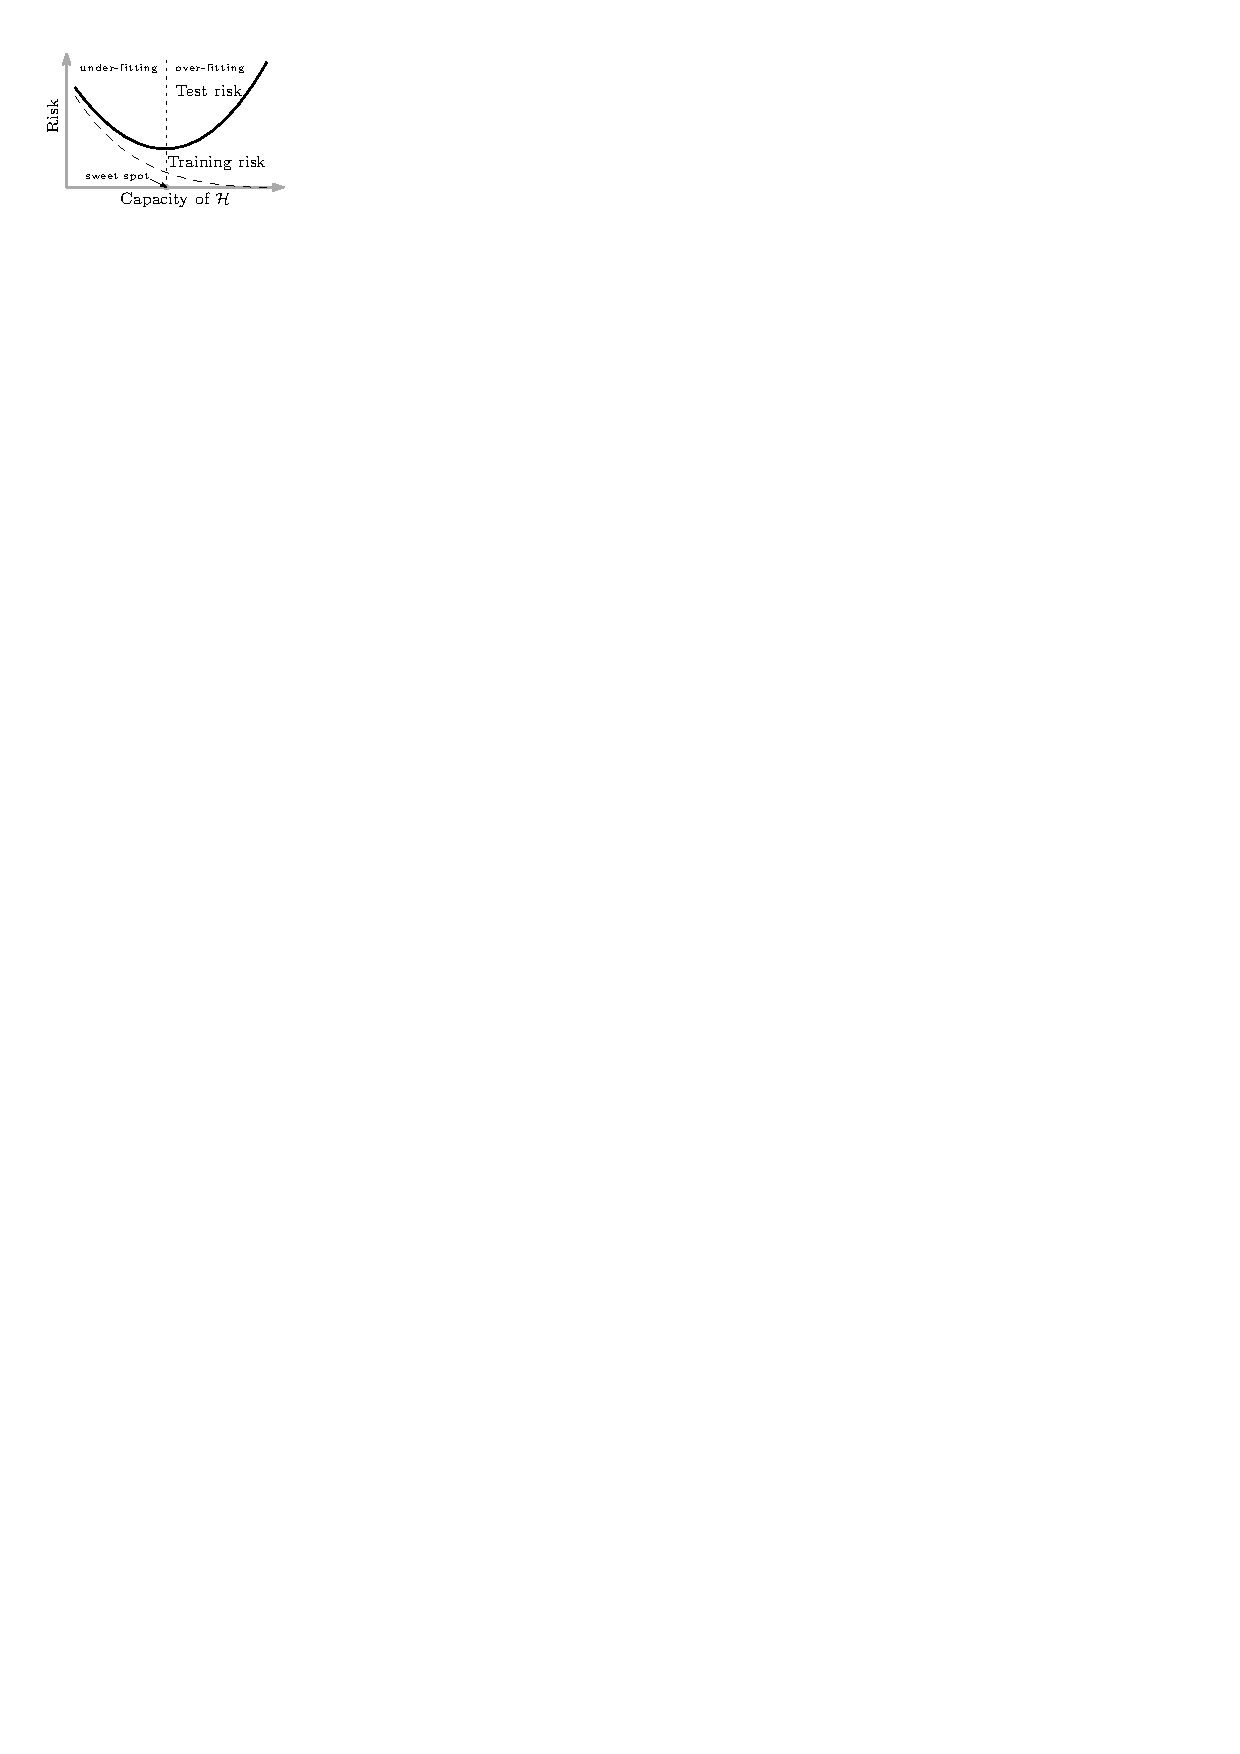
\includegraphics[height=0.13\textheight]{pdf/u-shaped.pdf} &
    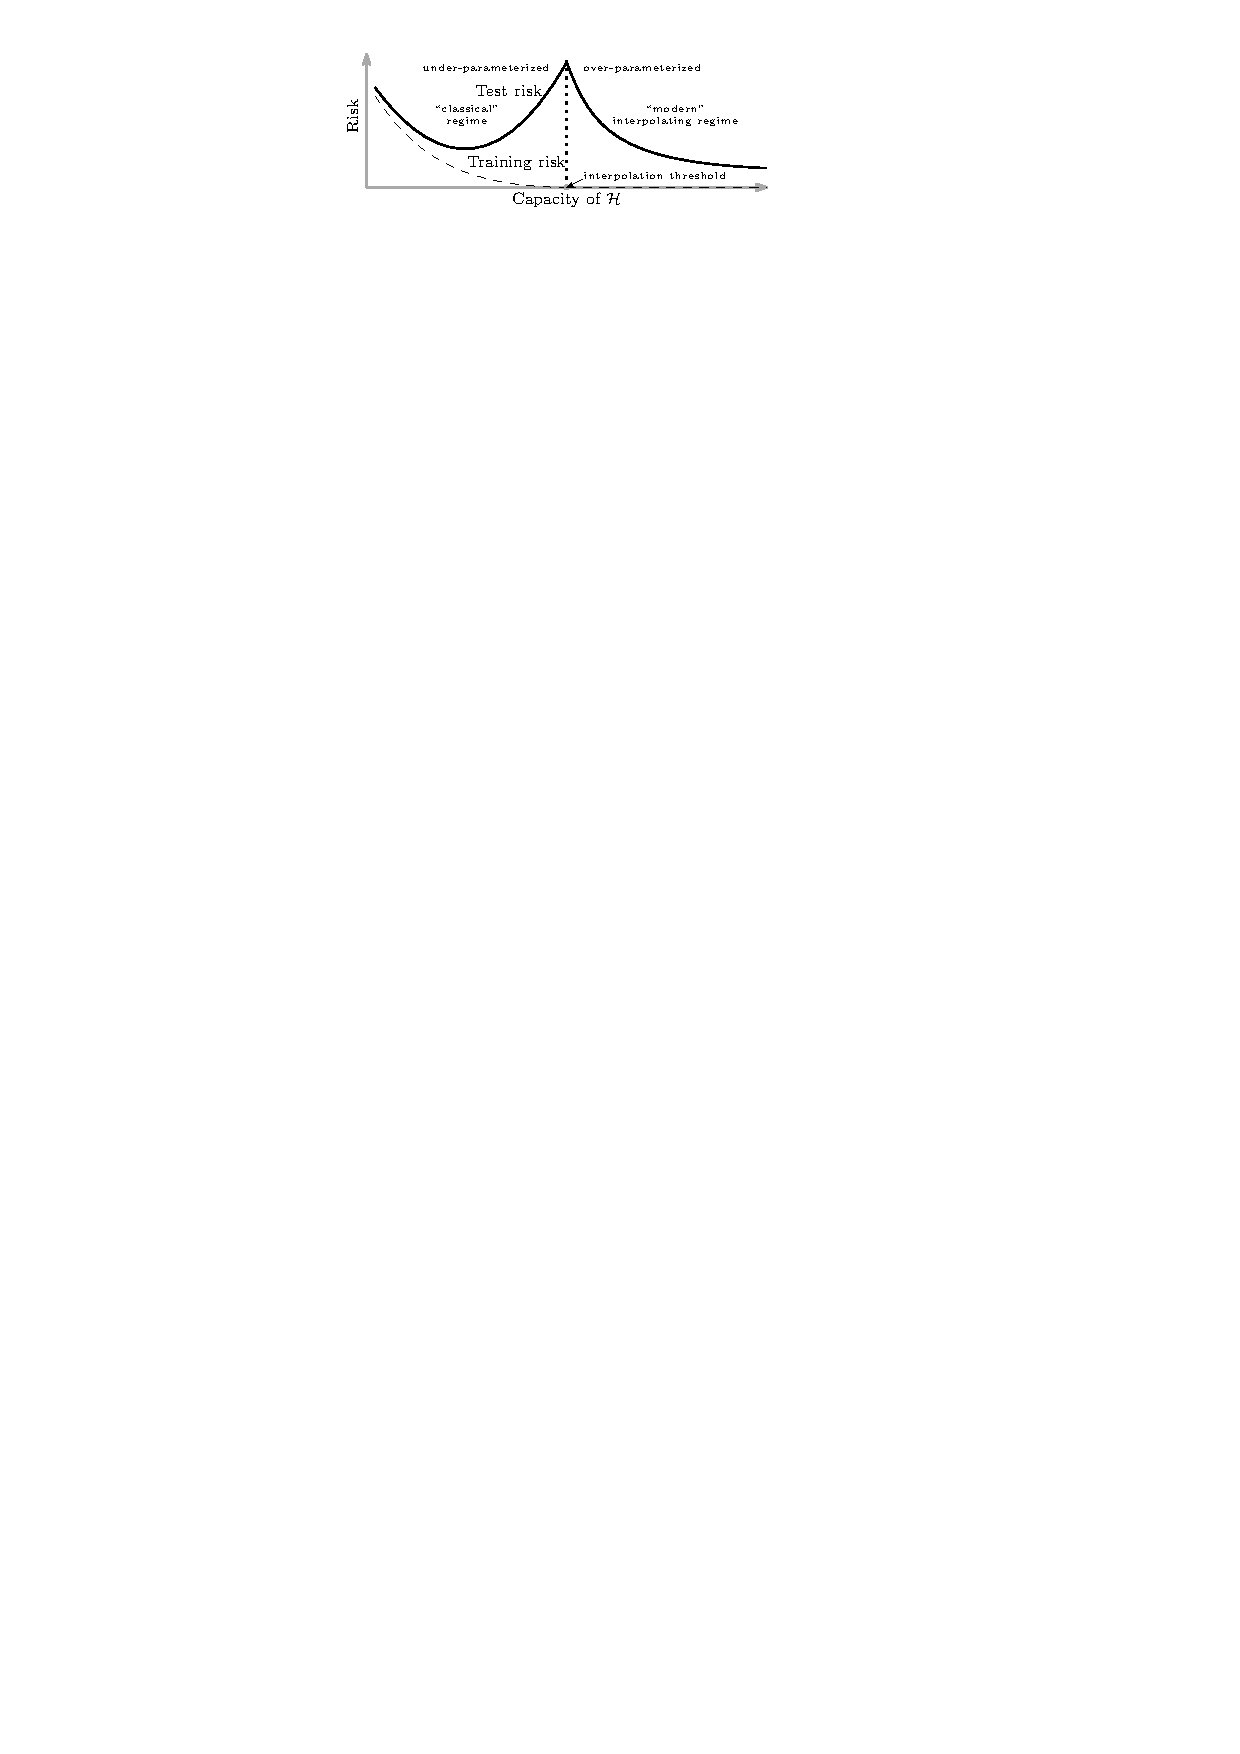
\includegraphics[height=0.13\textheight]{pdf/doubledescent.pdf} \\
    {\bf (a)} & {\bf (b)}
    \end{tabular}
    \caption{{\small {\bf Curves for training risk (dashed line) and test risk (solid line).}
      ({\bf a}) The classical \emph{U-shaped risk curve} arising from the bias-variance trade-off.
      ({\bf b}) The \emph{double descent risk curve}, which incorporates the U-shaped risk curve (i.e., the ``classical'' regime) together with the observed behaviour from using high capacity function classes (i.e., the ``modern'' interpolating regime), separated by the interpolation threshold.
      The predictors to the right of the interpolation threshold have zero training risk. Reproduced from \cite{belkin_reconciling_2019}.}}
    \label{fig:double-descent}
\end{figure*}

The main finding that Belkin found is a pattern for how the apparent performance on unseen data depends on model capacity and the mechanism underlying the emergence of double descent. When function class capacity is below the "interpolation threshold", learned predictors exhibit the classical $U$-shaped curve from Figure~\ref{fig:double-descent}. The `modern' interpolating regime marks the opposite trend to the right, where the risk starts to decrease up to a lower bound, which then can be called the \textit{optimal descent bound}. 

\blockquote[\cite{belkin_reconciling_2019}]{The bottom of the $U$ is achieved at the sweet spot which balances the fit to the training data and the susceptibility to over-fitting:
to the left of the sweet spot, predictors are under-fit, and immediately to the right, predictors are over-fit.
When we increase the function class capacity high enough (e.g., by increasing the number of features or the size of the neural network architecture), the learned predictors achieve (near) perfect fits to the training data---i.e., interpolation.
Although the learned predictors obtained at the interpolation threshold typically have high risk, we show that increasing the function class capacity beyond this point leads to decreasing risk, typically going below the risk achieved at the sweet spot in the ``classical'' regime.}

At this point, we would like to also clarify the term interpolation threshold in this case. Usually, under the pretext of overfitting and underfitting, interpolation threshold means the following: 

\begin{definition}[Interpolation threshold]
    Assuming a typical supervised learning setting, for a hypothesis $h$ within class structure $\mathcal{H}$, and a supposed concept $c$ of the class $\mathcal{C}$. Suppose $[X,Y]\subset c\in \mathcal{C}$ being the dataset, or \textit{observable space} of $c$ on which $h$ is tested on. Under the \textbf{empirical generalization learning} procedure, partitioning $[X,Y]$ into $[X,Y]_{1}$ and $[X,Y]_{2}$, for error evaluated on the first set, $\hat{R}_{1}(h)$ called training error, and the second set, $\hat{R}_{2}(h)$ called test error, with optimization applied on the first set, then evaluated statically on the second, the \textbf{interpolation threshold} with respect to a particular complexity measure of $h$, $\mathcal{M}(h)$, is the point $\mathcal{M}_{0}(h)$ where it is possible for $\hat{R}_{2}(h)/\hat{R}_{1}(h)\approx 1$, for $\hat{R}_{1}(h)\ll \epsilon$, $\hat{R}_{2}(h)\ll \epsilon$, with $\epsilon \geq 0$. 
\end{definition}

This basically means that what is learnt, with respect to the model complexity that gauge \textit{how much} and \textit{what} the model can learn, perfectly fits the concept $c$ itself, from the observation space on its own. We can say that, that specific sense, we gain the assumption that the observation space is \textit{fully representative} of the concept class, and the concept class is then fully realized by the model. Such point where that is possible, or there then such behaviour is possible, is called the interpolation point. The definition relies on the statement `where it is possible', hence it still, does not give us a particularly sound notion on to how and what constitute such possibility. The term empirical generalization learning comes from the fact that the procedure in practice of estimating and optimizing train-test-validation set in itself, is an imperfect empirical approximation of generalization testing. While the fact that we cannot gauge generalization error, in a purely blind black-box setting is settled (\cite{10.5555/2371238,10.5555/2930837,10.5555/2621980}), the method is then to try to mimic such by using generalization-via-hidden observations. To facilitate this, deliberately, the empirical learning procedure is only dynamic during training session, and static throughout the whole testing and validation testing section, and further on. 

By default, in general theory, such interpolating point is dangerous. Not only because it is inherently difficult to know exactly what the dataset constitute, whether it is actually representative of the concept that gives rise to it, or the structural information, noises, and interferences in between. It is hence impossible, to a certain point, to truly know the effectiveness of the model beside interpolating the current dataset which forms the observable details. 

Another prominent discovery to look at is \cite{nakkiran_deep_2019}, on the double descent of deep learning models. The paper serves as the first observation upon which double descent is observed on modern, deep learning theoretic models, especially complex one like Transformer or ResNet networks. 

They define \emph{effective model complexity} of $\mathcal{T}$ (w.r.t. distribution $\mathcal D$) to be the maximum number of samples $n$ on which $\mathcal{T}$ achieves on average $\approx 0$ \emph{training error}. This is an entirely empirical definition, similarly per definition as VC-dimension. 

\newcommand{\EMC}{\mathrm{EMC}}
\begin{definition}[Effective Model Complexity]
The \emph{Effective Model Complexity} (EMC) of a training procedure $\cT$, with respect to distribution $\cD$ and parameter $\epsilon>0$,
is defined as:
\begin{align*}
    \EMC_{\cD,\eps}(\cT)
    :=  \max \left\{n ~|~ \E_{S \sim \cD^n}[ \mathrm{Error}_S( \cT( S )  ) ] \leq \eps \right\}
    \end{align*}
    where $\mathrm{Error}_S(M)$ is the mean error of model $M$ on train samples $S$.
\end{definition}

Using this definition, their main hypothesis can then be stated as the following three-fold regions:

\begin{hypothesis}[Generalized Double Descent hypothesis, informal] \label{hyp:informaldd}
For any natural data distribution $\cD$, neural-network-based training procedure $\cT$, and small $\epsilon>0$,
if we consider the task of predicting labels based on  $n$ samples from $\cD$ then:
\begin{description}
    \item[Under-parameterized regime.]  If~$\EMC_{\cD,\epsilon}(\cT)$ is sufficiently smaller than $n$, any perturbation of $\cT$ that increases its effective complexity will decrease the test error.
    \item[Over-parameterized regime.] If $\EMC_{\cD,\epsilon}(\cT)$ is sufficiently larger than $n$,
    any perturbation of $\cT$ that increases its effective complexity will decrease the test error.
    
    \item[Critically parameterized regime.] If $\EMC_{\cD,\epsilon}(\cT) \approx n$, then
    a perturbation of $\cT$ that increases its effective complexity
    might decrease {\bf or increase} the test error.
\end{description}
\end{hypothesis}

It is to notice that this definition is also only observational. By that, it only outlines the specific region of interest where the paradigm shift is identified through experimental results. It has no effective predictive power, or rather descriptive power more than setting up hypothesis with respect to the effective model complexity, and some arbitrary perturbation. \cite{nakkiran_deep_2019} also noticed this difficulty in providing a theoretical definition and theorem regarding such hypothesis, as said in their manuscript. The existence of the critical regime is also not defined. 

The behaviour itself has been particularly investigated, in certain settings. For example, before \cite{belkin_reconciling_2019}, \cite{advani2017highdimensionaldynamicsgeneralizationerror} investigated the generalization error in neural networks of high-dimensional measure. Of such, various behaviours that bear similarity to double descent can be observed. \cite{belkin2018understanddeeplearningneed} expanded on his previous research on the particular subset of kernel learning models, providing a theoretical analysis of specifically the Laplacian kernel on standard neural network. \cite{mei2020generalizationerrorrandomfeatures} investigated random feature regression in such regard, and also found similar results. 

The fact that double descent is not well-defined itself is a problem on its own. Up to the author's knowledge and of myself, there has been no effective definition or given description that outlines specifically how double descent can be structured. Instability in reproducing experiments and the effective range of the phenomena remains a question on its own. 




\clearpage

\nocite{*}
\printbibliography

\end{document}